\label{Free energy and the effective action}
The theory in this section is based on \cite{Peskin:IntroQFT,weinberg_1995,weinberg_1996_vol2,Schwartz:QFT}.
Feynman diagrams are drawn using JaxoDraw~\cite{JaxoDraw}.

\subsection{QFT via path integrals}
\label{section:path integral}
The vacuum transition amplitude is given by the path integral
\begin{equation}
    Z = \lim_{T\rightarrow \infty} \braket{\Omega, T/2}{-T/2, \Omega}
    = \lim_{T\rightarrow \infty} \inner{\Omega}{ e^{-iHT} }{\Omega}
    = \int \D \pi \D \varphi \, \exp{ i \int \dd^4 x \, \left(\pi \dot \varphi - \He[\pi, \varphi]\right) },
\end{equation}
where $\ket{\Omega}$ is the vacuum of the theory.
By introducing a source term into the Hamiltonian density, $\He \rightarrow \He - J(x)\varphi(x)$, we get the generating functional
\begin{equation}
    Z[J] = 
    \int \D \pi \D \varphi \, 
    \exp{ i \int \dd^4 x \, \left(\pi \dot \varphi - \He[\pi, \varphi]+ J\varphi\right) }.
\end{equation}
If $\He$ is quadratic in $\pi$, we can complete the square and integrate out $\pi$ to obtain
\begin{equation}
    Z[J] = C \int \D \varphi \, \exp{i \int \dd^4 x\, (\Ell[\varphi] + J \varphi)}.
\end{equation}
$C$ is infinite, but constant, and will drop out of physical quantities.
In scattering theory, the main objects of study are correlation functions $\ex{\varphi(x_1)\varphi(x_2)...} = \inner{\Omega}{T\left\{\varphi(x_1)\varphi(x_2)\dots\right\}}{\Omega}$, where $T$ is the time ordering operator.
These are given by functional derivatives of $Z[J]$, 
\begin{equation}
    \label{correlator from generating functional}
    \ex{\varphi(x_1)\varphi(x_2)...}
    = 
    \frac{\int \D \varphi(x)\,  (\varphi(x_1)\varphi(x_2)...) e^{i S[\varphi]}}
        {\int \D \varphi(x)\, e^{i S[\varphi]}}
    =
    \frac{1}{Z[0]} \prod_i\left( -i  \fdv{J(x_i)}\right) Z[J]\Big|_{J = 0},
\end{equation}
where 
\begin{equation}
    S[\varphi] = \int \dd^4 x \, \Ell[\varphi]
\end{equation}
is the action of the theory.
The functional derivative is described in \autoref{section:Functional derivative}.
In a free theory, we are able to write
\begin{equation}
    Z_0[J] = Z_0[0] \exp(i W_0[J]), \quad 
    W_0[J] = \frac{1}{2} \int \dd^4 x \dd^4 y \, J(x) D_0(x - y) J(y),
\end{equation}
where $D_0$ is the propagator of the free theory.
Using this form of the generating functional, \autoref{correlator from generating functional} becomes
\begin{align*}
    & \frac{1}{Z[0]}  (-i)^n\fdiff{}{J(x_1)} ... \fdiff{}{J(x_n)} Z_0[J]  \Big|_{J = 0}
    = (-i)^n \fdiff{}{J(x_1)} ... \fdiff{}{J(x_n)} e^{i W_0[J]} \Big|_{J = 0}\\
    & = (-i)^{n} \fdiff{}{J(x_1)} ... \fdiff{}{J(x_{n-1})} \left(i \fdiff{W_0[J]}{ J(x_{n}) } \right) e^{i W_0[J]} \Big|_{J = 0}\\
    & = (-i)^{n}\fdiff{}{J(x_2)} ... \fdiff{}{J(x_{n-1})}
    \left(
        i\fdiff{ W_0[J] }{ J(x_{n-1}), J(x_{n}) }
        + i^2 \fdiff{W_0[J]}{J(x_{n-1})} \fdiff{W_0[J]}{J(x_{n})}
    \right) 
    e^{i W_0[J]} \Big|_{J = 0}
    = \dots \\
    &= 
    (- i )^{n/2}\sum_{{(a, b)}} \prod_{i=1}^{n/2}
    \fdiff{ W_0[J] }{ J(x_{a(i)}), J(x_{b(i)}) } \Big|_{J = 0}.
\end{align*}
In the last line we have introduced the functions $a, \, b$ which define a way to pair up $n$ elements.
The domain of the functions are the integers between $1$ and $n/2$, the image a subset of the integers between $1$ and $n$ of size $n/2$.
A valid pairing is a set $\{(a(1), b(1)), \dots (a(n/2), b(n/2))\}$, where all elements $a(i)$ and $b(j)$ are different, such all integers up to and including $n$ are featured.
A pair is not directed, so $(a(i), b(i))$ is the same pair as $(b(i), a(i))$.
The sum is over the set ${\{(a, b)\}}$ of all possible, unique pairings.
If $n$ is odd, the expression is equal to $0$.
This is Wick's theorem, and it can more simply be stated as \emph{a correlation function is the sum of all possible pairings of 2-point functions},
\begin{equation}
    \ex{{\prod}_{i=1}^{n} \varphi(x_i)  }_0
    = \sum_{\{(a, b)\}}  \prod_{i=1}^n  \ex{\varphi(x_{a(i)}) \varphi(x_{b(i)})}_0.
\end{equation}
The subscript on the expectation value indicates that it is evaluated in the free theory.

If we have an interacting theory, that is a theory with an action $S = S_0 + S_I$, where $S_0$ is a free theory, the generating functional can be written
\begin{equation}
    \label{partition function of interacting theory.}
    Z[J] 
    = Z_0[0] \ex{\exp(iS_I + i\int \dd^4 x \, J(x) \varphi(x))}_0.
\end{equation}
We can expand the exponential in power series, which means the expectation in \autoref{partition function of interacting theory.} becomes
\begin{equation}
    \sum_{n, m} \frac{1}{n! m!} \ex{(iS_I)^n \left(i\int \dd^4 x \, J(x) \varphi(x)\right)^m}_0.
\end{equation}
The terms in this series are represented by Feynman-diagrams, which are constructed from the Feynman-rules, and can be read from the action.
We will not go into further details on how the Feynman-rules are derived, which can be found in any of the main sources for this section~\cite{Peskin:IntroQFT,weinberg_1995,weinberg_1996_vol2,Schwartz:QFT}.
The source terms gives rise to an additional vertex
\begin{equation}
    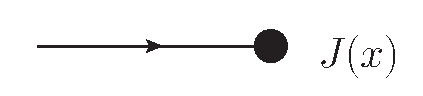
\includegraphics[width=0.25\textwidth, valign=c]{figurer/feynman-diagram/cnt_vertex.eps}.
\end{equation}
The generating functional $Z[J]$ equals $Z_0[0]$ times \emph{the sum of all diagrams with external sources $J(x)$}.
% The expectation value
% \begin{equation}
%     \ex{(iS_I)^n (\varphi(x)J(x))^m}_0
% \end{equation}
% are all diagrams with $n$ vertices given by the Feynman rules from the interacting action $S_I$, as well as $m$ m source vertices.

Consider a general diagram without external legs, built up of $N$ different connected subdiagrams, where subdiagram $i$ appears $n_i$ times.
As an illustration, a generic vacuum diagram in $\phi^4$-theory has the form
\begin{align}
    \label{Feinman diagrams}
    V = 
    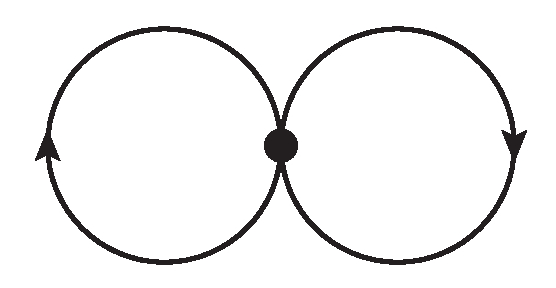
\includegraphics[width=0.1\textwidth, valign=c]{figurer/feynman-diagram/phi-4_loop_notext.eps}
    \times
    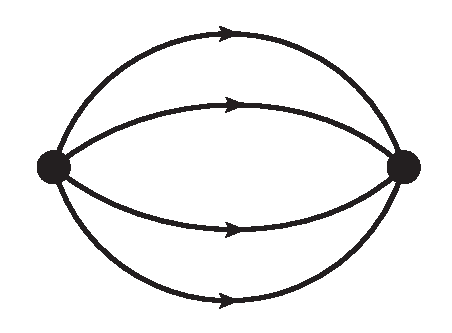
\includegraphics[width=0.08\textwidth, valign=c]{figurer/feynman-diagram/phi-4_2_loop.eps}
    \times
    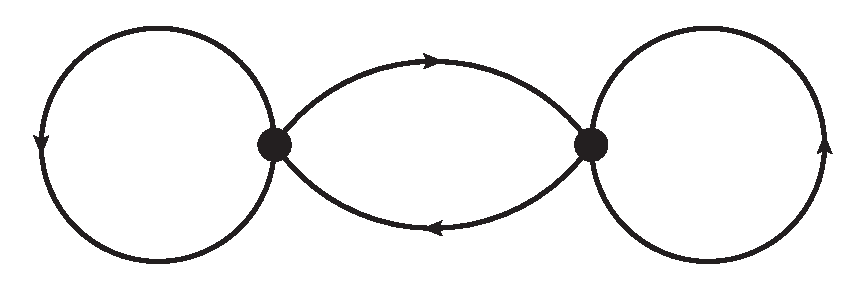
\includegraphics[width=0.14\textwidth, valign=c]{figurer/feynman-diagram/phi-4_2_loop2.eps}
    \times
    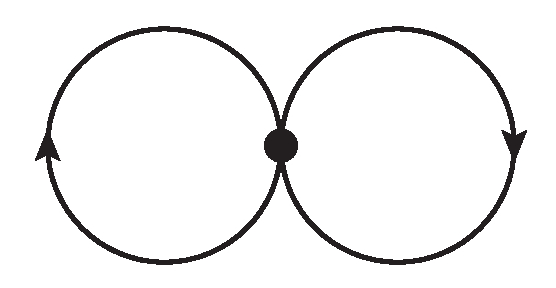
\includegraphics[width=0.1\textwidth, valign=c]{figurer/feynman-diagram/phi-4_loop_notext.eps}
    \times \dots.
\end{align}
If sub-diagram $i$ as a stand-alone diagram equals $V_i$, then each copy of that subdiagram contribute a factor $V_i$ to the total diagram.
However, due to the symmetry of permuting identical subdiagrams, one must divide by the extra symmetry factor $s = n_i !$, which is the total number of permutation of all the copies of diagram $i$.
The value of the total diagram is therefore
\begin{align}
    \label{Feynman diagrams}
    V
    = \prod_{i= 1}^N \frac{1}{n_i!} V_i^{n_i}.
\end{align}
$V$ is uniquely defined by a finite sequence of integers, $(n_1, n_2, \dots n_N, 0, 0, \dots)$, so the sum of all diagrams is the sum over the set $S$ of all finite sequences of integers.
This allows us to write the sum of all diagrams as
\begin{equation}
    \label{sum of all diagrams}
    \sum_{(n_1, ...)\in S} \prod_{i} \frac{1}{n_i!} V_i^{n_i}
    = \prod_{i = 1}^{\infty} \sum_{n_i=1}^{\infty} \frac{1}{n_i!} V_i^{n_i}
    = \exp({\sum}_i V_i).
\end{equation}
We showed that the generating functional $Z[J]$ were the $Z_0[0]$ times the sum of all diagrams due to external sources.
Using \autoref{sum of all diagrams}, we see that the sum of all \emph{connected} diagrams $W[J]$ is given by
\begin{equation}
    Z[J] = Z_0[0]\exp(i W[J]).
\end{equation}
We can see that this is trivially true for the free theory, the only connected diagram is
\begin{equation}
    W_0[J] = 
    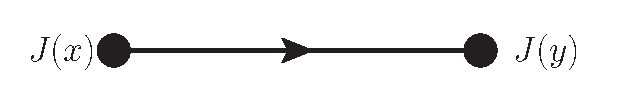
\includegraphics[valign=c, width=0.3\textwidth]{figurer/feynman-diagram/current-current.eps}.
\end{equation}
